% Test tex file!

\documentclass[a4paper,12pt]{article}
\usepackage{times}  % DO NOT CHANGE THIS
\usepackage{helvet} % DO NOT CHANGE THIS
\usepackage{courier}  % DO NOT CHANGE THIS
\usepackage[hyphens]{url}  % DO NOT CHANGE THIS
\usepackage{graphicx} % DO NOT CHANGE THIS
\urlstyle{rm} % DO NOT CHANGE THIS
\def\UrlFont{\rm}  % DO NOT CHANGE THIS
\usepackage{natbib}  % DO NOT CHANGE THIS AND DO NOT ADD ANY OPTIONS TO IT
\usepackage{caption} % DO NOT CHANGE THIS AND DO NOT ADD ANY OPTIONS TO IT
\frenchspacing  % DO NOT CHANGE THIS
\setlength{\pdfpagewidth}{8.5in}  % DO NOT CHANGE THIS
\setlength{\pdfpageheight}{11in}  % DO NOT CHANGE THIS
\usepackage{algorithm} %format of the algorithm 
\usepackage{algorithmic} %format of the algorithm 
\usepackage{multirow} %multirow for format of table 
\usepackage{amsmath} 
\usepackage{xcolor}
\usepackage{amssymb}
\usepackage{amsmath}
\usepackage{CJKutf8}
\usepackage{courier}

\begin{document}

\begin{CJK}{UTF8}{gbsn}
% \begin{CJK}{UTF8}{gkai}

\title{强化学习:作业四}

\author{傅浩敏 MG20370012}

\date{2020年12月28日}

\maketitle

\section{作业内容}
本实验需要在gridworld环境中实现model-based Q-learning算法并评估算法性能。本实验的gradworld是一个8*8的迷宫,agent需要拿到位于(0,7)处的钥匙后到达终点才算通关,因此环境输出了状态除了当前坐标外还包含了是否获得钥匙这一额外特征。本次实验由三部分组成,首先我们实现Dyna-Q算法,并且调整超参数以尽可能达到算法可提升的性能极限。第二部分是使用神经网络来预测环境model,同样通过调整超参数来获得最佳的性能表现。第三部分是改进model学习过程以应对稀疏奖励的问题,并且分析这些改进对算法带来了哪些变化。最后需要分析不同的学习方式和超参数对model-based算法性能的影响,并且讨论产生这些影响的可能的原因。

\section{实现过程}
\subsection{算法描述}
首先需要在 \texttt{algo.py} 中实现Q-learning Agent。在本实验中我直接使用HW2中实现过的Q-learning算法,我以表格的形式记录Q值并且动态地向Q表中添加新的状态-动作对。

对于普通的Dyna-Q算法,我也采用表格的形式记录状态-动作-新状态之间的转移关系。每当在环境中采样后,需要将采样到的转移关系存在转移表中。我们需要同时使用采样到的转移和转移表中储存的转移来更新Q表。

在第二个实验中,我们使用神经网络来预测状态-动作-新状态之间的转移关系,在环境中采样后都要把采样到的转移关系存储在buffer中。每经过若干轮迭代,我们从buffer中抽取若干样本来训练我们的model。同样的,我们需要同时使用采样到的转移关系和神经网络模型预测的转移关系来更新Q表。

在第三个实验中,我们对model的学习过程进行了一些改进。首先,我们在采样的同时记录了那些获得钥匙的关键转移。在训练神经网络模型时,固定这些样本在训练样本中的比例,从而保证model始终能够对“是否获得钥匙”做出正确的预测。第二个改进是在Q表中的值超过某个定义的上下界时进行截断。
\subsection{代码实现}
Algorithm 1 为Dyna-Q的伪代码:
\begin{algorithm}[!h]
	\caption{Dyna-Q}
	\begin{algorithmic}[1]
		\STATE Initial $Q_\pi$ and $Model$. Given reword function $R$, and terminal function $D$. Given learning rate $\alpha$, discount rate $\gamma$, and repeat number $n$.
		\FOR{$1,2,\cdots$}
		\STATE $s=env.reset()$
		\FOR{$1,\cdots,steps$}
		\STATE  epsilon-greedy: $a=\pi_\epsilon(s)$
		\STATE interact with environment: $s',r,done=env.step(a)$
		\STATE update Q: $Q_\pi(s,a)+=\alpha(r+\gamma(1-done)\max_{a'} Q_\pi(s',a')-Q_\pi(s,a))$
		\STATE update Model: $Model(s,a)\leftarrow r,s'$
		\STATE $s=s'$
		\IF{$done$}
		\STATE $s=env.reset()$
		\ENDIF
		\ENDFOR
		\FOR{$1,2,\cdots,n$}
		\STATE $s_m,a_m,s'_m=$ random sample from ovserved transitions
		\STATE get reword and done: $r_m=R(s_m,a_m,s'_m),d_m=D(s_m,a_m,s'_m)$
		\STATE update Q: $Q_\pi(s_m,a_m)+=\alpha(r_m+\gamma (1-d_m)\max_{a'_m} Q_\pi(s'_m,a'_m)-Q_\pi(s_m,a_m))$
		\ENDFOR
		\ENDFOR
	\end{algorithmic}
\end{algorithm}

Algorithm 2 为实验3的伪代码。可以通过删除与sensitive buffer和clip函数相关的语句来获得实验2的伪代码,因此实验2的代码不再单独列出:
\newpage
\begin{algorithm}[H]
	\caption{Neural Network Algorithm with Improvement}
	\begin{algorithmic}[1]
		\STATE Initial $Q_\pi$, $Model$, transition buffer $Buffer$, and sensitive buffer $Buffer_s$. Given reword function $R$, terminal function $D$, and clip function $clip$. \\Given learning rate $\alpha$, discount rate $\gamma$, repeat time $n$, learning period $m$, step length $h$, and start time $start\_planning$.
		\FOR{$1,2,\cdots$}
		\STATE $s=env.reset()$
		\FOR{$1,\cdots,steps$}
		\STATE epsilon-greedy: $a=\pi_\epsilon(s)$
		\STATE interact with environment: $s',r,done=env.step(a)$
		\STATE update Q: $Q_\pi(s,a)+=\alpha(r+\gamma(1-done)\max_{a'} Q_\pi(s',a')-Q_\pi(s,a))$
		\STATE clip Q: $Q_\pi(s,a)=clip(Q_\pi(s,a),-100,100)$
		\STATE update buffer: $Buffer.append(s,a,r,s')$
		\IF{$s[-1] \neq s'[-1]$}
		\STATE update sensitive buffer: $Buffer_s.append(s,a,r,s')$
		\ENDIF
		\STATE $s=s'$
		\IF{$done$}
		\STATE $s=env.reset()$
		\ENDIF
		\ENDFOR
		\FOR{$1,2,\cdots,m$}
		\STATE $transition\_list=$ sample transition from $Buffer$ and $Buffer_s$
		\STATE train model: $Model.train\_transition(transition\_list)$
		\ENDFOR
		\IF{$iter>start\_planning$}
		\FOR{$1,2,\cdots,n$}
		\STATE $s_m=$ random sample from ovserved transitions
		\FOR{$1,2,\cdots,h$}
		\STATE epsilon-greedy: $a_m=\pi_\epsilon(s_m)$
		\STATE calcualte next state: $s'_m=Model(s_m,a_m)$
		\STATE get reword and done: $r_m=R(s_m,a_m,s'_m),d_m=D(s_m,a_m,s'_m)$
		\STATE update Q: $Q_\pi(s_m,a_m)+=\alpha(r_m+\gamma (1-d_m)\max_{a'_m} Q_\pi(s'_m,a'_m)-Q_\pi(s_m,a_m))$
		\STATE clip Q: $Q_\pi(s_m,a_m)=clip(Q_\pi(s_m,a_m),-100,100)$
		\IF{$d_m$}
		\STATE $break$
		\ENDIF
		\ENDFOR
		\ENDFOR
		\ENDIF
		\ENDFOR
	\end{algorithmic}
\end{algorithm}
\section{复现方式}
首先在主文件夹下运行 \texttt{pip install -r requirements.txt} 安装依赖,如果已安装依赖也可跳过此步骤\footnote{注意到原始代码使用的tensorflow版本是v1,但是本机只安装了v2版本的tensorflow,因此我开启了兼容模式。如果运行出错可能需要在 \texttt{code4/algo.py} 中还原tensorflow的import方式}。在 \texttt{code4} 文件夹下运行 \texttt{python main.py --model=dyna} 可以开始Dyna-Q的实验。将参数 \texttt{--model} 设置为 \texttt{nn} 或 \texttt{advnn} 可以开始实验二或实验三。设置 \texttt{--m --n --h --sp} 可以修改对应的实验参数。其中 \texttt{--sp} 对应start\_planning参数。
\subsection{参数介绍}
实验中涉及的主要参数见Table 1, "*" 表示该参数的值会在实验中改变。
\begin{table}[!h]
	\renewcommand{\arraystretch}{1.2}
	\caption{主要参数}
	\centering
	\begin{tabular}{ccc}
		\hline
		名称& 默认值& 说明\\
		\hline
		learning\_rate& 0.2 & 学习率 $\alpha$\\
		gamma& 0.99 & 折扣系数 $\gamma$\\
		epsilon& 0.2 & 探索概率 $\epsilon$ \\
		frames& 10000 & 训练总帧数\\
		n& * & model中采样次数\\
		m& * & model训练次数\\
		h& * & model采样时的步长\\
		start\_planning& * & 开始从model中采样的帧数\\
		\hline
	\end{tabular}
\end{table}
\section{实验效果}
\subsection{实验一}
从n=0开始,每次将n增大600,找到大致的最优值范围,然后进行细微调整,找到的经验性$n^*$的估计大致在1500左右。实验中的其他主要参数设置为:m=0, h=1, start\_planning=0。我发现在model free的情况下,policy大概在9000步左右收敛,在n超过1500时,策略收敛所需的步长不会再明显下降。具体实验结果如下:
\begin{table}[H]
	\renewcommand{\arraystretch}{1.2}
	\caption{n与策略收敛时间和消耗样本量的大致关系}
	\centering
	\begin{tabular}{ccc}
		\hline
		n的取值& 收敛所需样本量& 收敛时间\\
		\hline
		0& 9200 & 20s\\
		600& 1800 & 05s\\
		1200& 1600 & 05s\\
		1400& 1300 & 05s\\
		\textbf{1500}& \textbf{800} & \textbf{03s}\\
		1800& 1000 & 04s\\
		2400& 900 & 04s\\
		3000& 1100 & 06s\\
		\hline
	\end{tabular}
\end{table}
部分实验中得分与使用样本量的关系如下:
\begin{figure}[htbp]
	\centering
	\begin{minipage}[t]{0.45\textwidth}
		\centering
		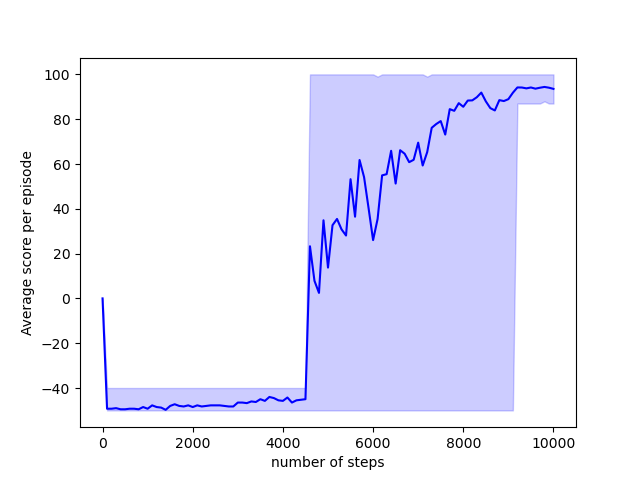
\includegraphics[width=6cm]{resource/n=0/performance.png}
		\caption{n=0}
	\end{minipage}
	\begin{minipage}[t]{0.45\textwidth}
		\centering
		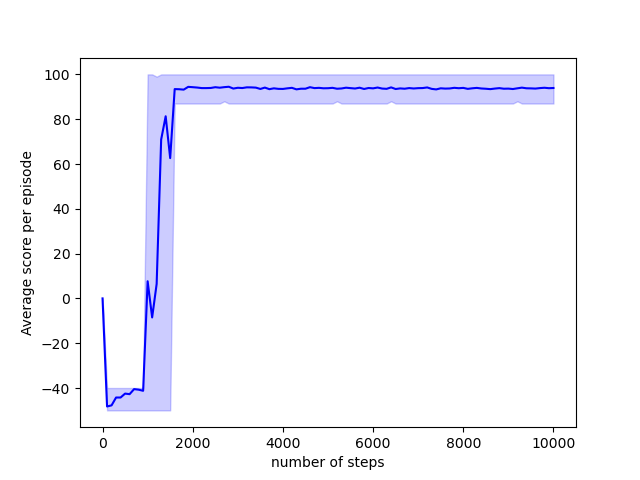
\includegraphics[width=6cm]{resource/n=1200/performance.png}
		\caption{n=1200}
	\end{minipage}
	\begin{minipage}[t]{0.45\textwidth}
		\centering
		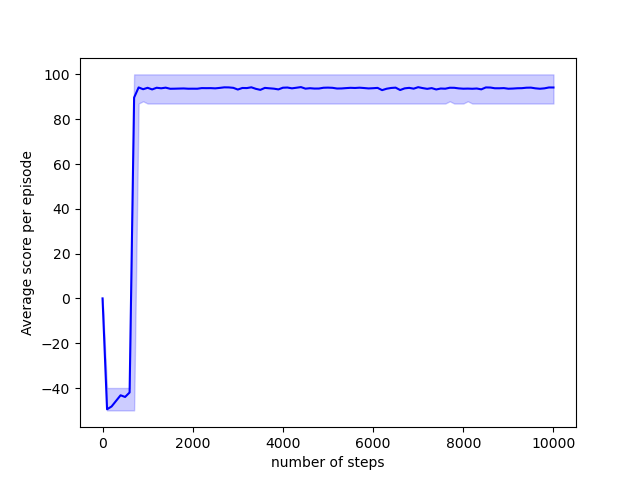
\includegraphics[width=6cm]{resource/n=1500/performance.png}
		\caption{\textbf{n=1500}}
	\end{minipage}
	\begin{minipage}[t]{0.45\textwidth}
	\centering
	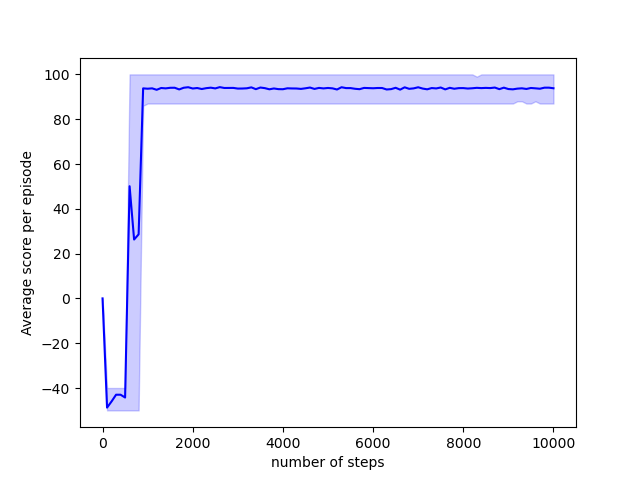
\includegraphics[width=6cm]{resource/n=2400/performance.png}
	\caption{n=2400}
\end{minipage}
\end{figure}
\newpage
\subsection{实验二}
我所找到的最好的参数组合是:n=300,m=1500,h=1,start\_planning=5。在此参数设置下,策略大约能稳定地在4000步左右收敛,并且收敛所需时间在一分钟之内。最优参数设置下的实验结果如下:
\begin{figure}[h!]
	\vspace{-0.3cm}
	\centering
	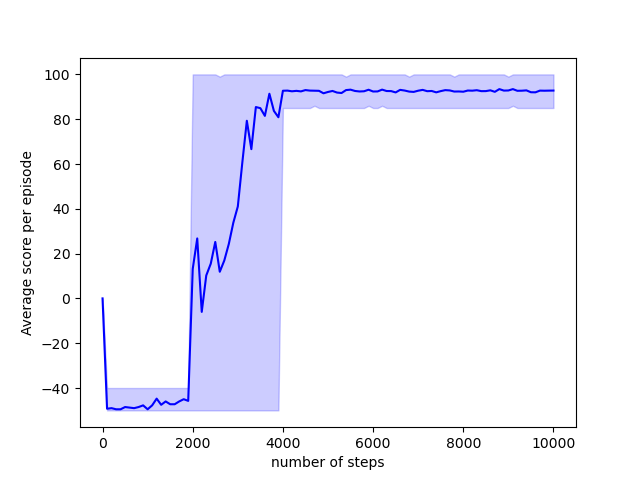
\includegraphics[width=7cm]{resource/n=300-m=1500-h=1-sp=5/performance.png}
	\caption{最优参数设置性能曲线}
\end{figure}
\\
同时,在最优参数设置的基础上,我分别改变了其他单一参数并进行了对比实验。修改的参数值和对应的实验结果如下:
\begin{figure}[htbp]
	\vspace{-0.3cm}
	\centering
	\begin{minipage}[t]{0.45\textwidth}
		\centering
		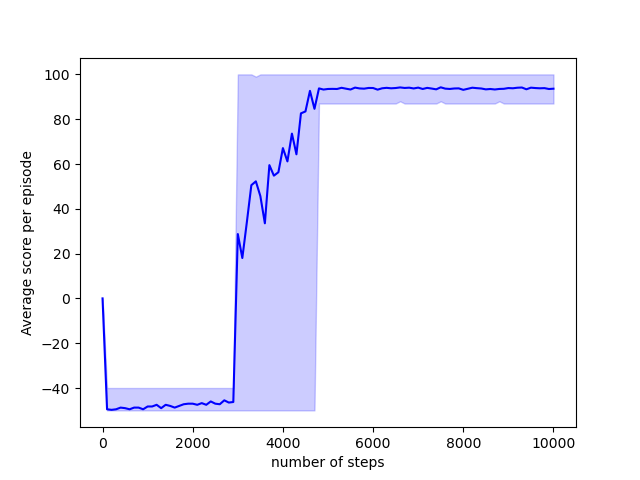
\includegraphics[width=6cm]{resource/n=100-m=1500-h=1-sp=5/performance.png}
		\caption{n=100}
	\end{minipage}
	\begin{minipage}[t]{0.45\textwidth}
		\centering
		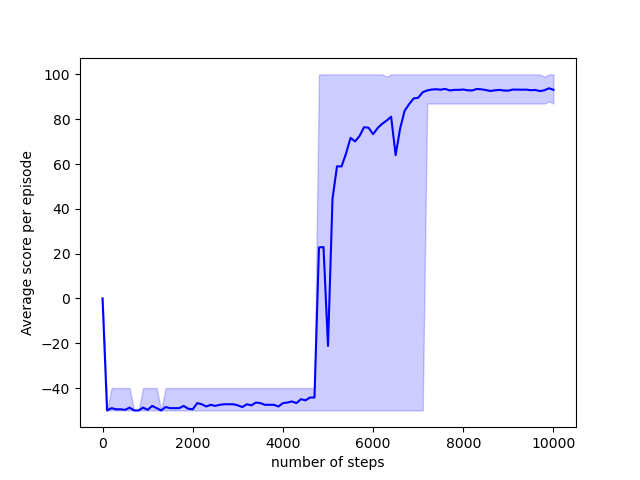
\includegraphics[width=6cm]{resource/n=300-m=500-h=1-sp=5/performance.png}
		\caption{m=500}
	\end{minipage}
	\begin{minipage}[t]{0.45\textwidth}
		\centering
		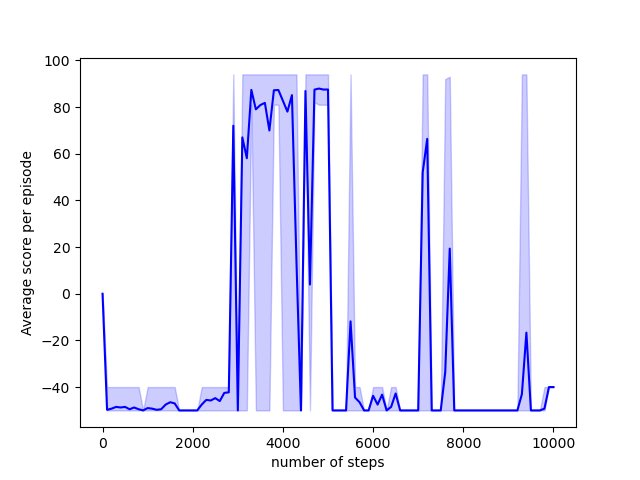
\includegraphics[width=6cm]{resource/n=300-m=1500-h=5-sp=5/performance.png}
		\caption{h=5}
	\end{minipage}
	\begin{minipage}[t]{0.45\textwidth}
		\centering
		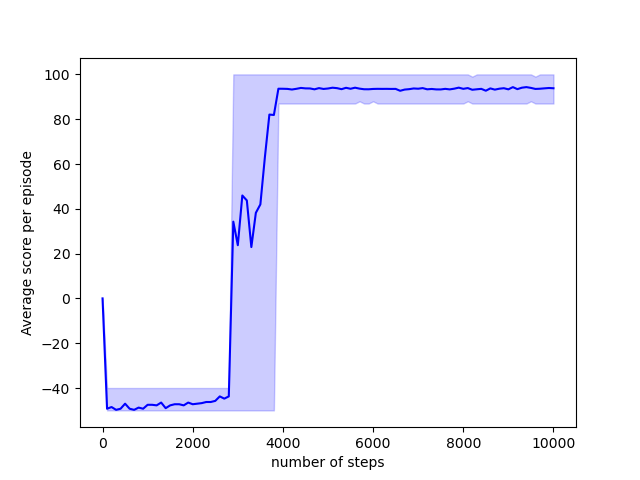
\includegraphics[width=6cm]{resource/n=300-m=1500-h=1-sp=0/performance.png}
		\caption{start\_planning=0}
	\end{minipage}
	\vspace{-1.5cm}
\end{figure}
\newpage
观察对比实验结果可以发现:仅减小n时,策略依然能够在5000步左右收敛,这说明在model学习良好的情况下,n对算法性能的影响不大。但是当我们减少model的学习次数m时,策略的收敛步数会有显著的降低,在7000多步时才能达到收敛状态。当我们改变在模型中采样的步长h时,算法性能会有很大的波动,这说明在model中进行持续采样产生的Compounding-Error会严重影响我们的训练过程。在本实验中,将从model中采样的开始时间start\_planning设置为0时,算法性能几乎不会改变。我认为这是由于本环境的model比较简单,神经网络在最初的几步迭代中也能把model学习得很好。

\subsection{实验三}
在对算法进行改进后我找到的最优参数组合变为:n=300,m=1000,h=1,\\start\_planning=5。在改进算法后,可以使用更小的m让策略在4000步左右收敛,收敛时间大约在一分钟左右。为了展示算法改进带来的效果,我使用上述参数设置对比了改进前后策略的性能曲线。我发现在m=1000时,改进前的算法在5000步左右才能收敛。具体的对比实验结果如下:
\begin{figure}[htbp]
	\centering
	\begin{minipage}[t]{0.45\textwidth}
		\centering
		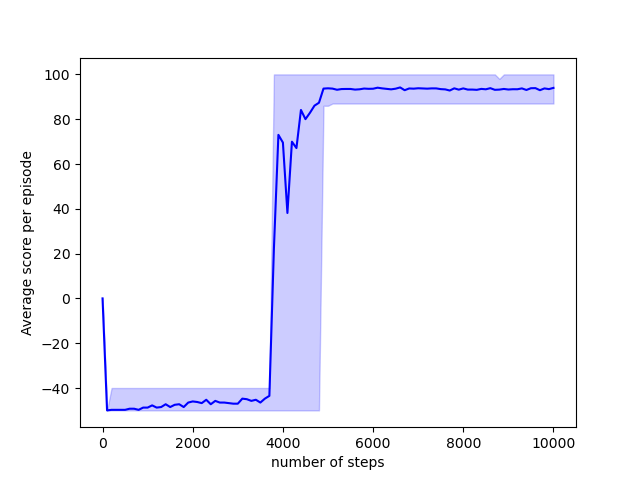
\includegraphics[width=6.5cm]{resource/nn-m=1000/performance.png}
		\caption{算法改进前}
	\end{minipage}
	\begin{minipage}[t]{0.45\textwidth}
		\centering
		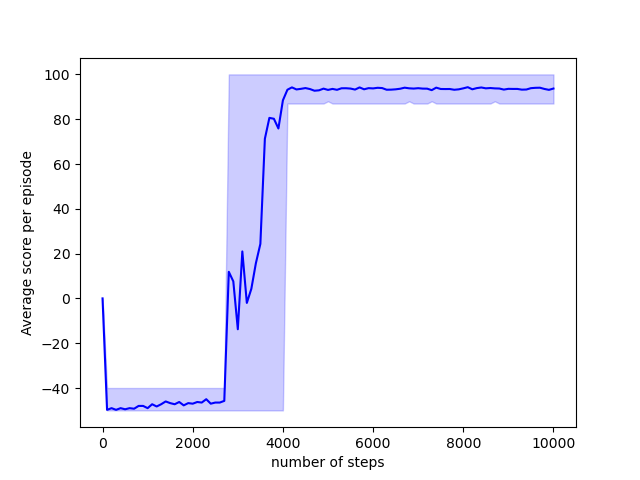
\includegraphics[width=6.5cm]{resource/advnn-m=1000/performance.png}
		\caption{算法改进后}
	\end{minipage}
\end{figure}
\\不过,我发现在Q表更新过程中没有Q值超出了[-100,100]这一上下界,因此我认为产生性能提升的原因是改进算法增加了sensitive buffer,而对Q值进行clip没有产生任何影响。
\section{问题讨论}
\paragraph{1.}根据上面实验,试讨论不同模型学习方式(table 和 neural network),不同参数对实验结果的影响和背后的原因,从而分析影响model-based的算法的性能的因素由哪些?


使用table学习模型可以直接学习到正确的转移,因此影响算法性能的主要参数是在模型中循环采样的次数n,在n足够大时我们就能获得最好的收敛步数,在此基础上我们仅需要考虑算法耗时。但使用神经网络学习model时,对环境的学习会存在一定的误差,而model的误差会严重影响Q表的更新效率。在这种情况下,提升模型中的采样次数n只会让我们的策略更加不稳定。我们必须首先保证神经网络能够较好的学习model,再利用由model产生的样本。

一个简单的方法是增加model的训练次数m,增强神经网络对环境的拟合度,但是过大的m会严重影响算法的效率。同时我们还需要保证在model中采样的步长h不能过大,避免产生累积误差影响Q表更新。注意到最初的几步迭代中,神经网络很有可能无法正确地学习到状态转移,因此可以通过延迟在model中采样的时间start\_planning来提升算法稳定性,不过这个方法在本实验中效果不明显。我们还可以为环境设计针对性的改进以提升model的训练性能。比如在本实验中,改变钥匙特征的转移样本数量较少但十分重要,如果直接采样神经网络可能会遗忘这些关键样本,因此加强对这一部分样本的学习能够提升model的学习效率。同时也许我们也可以人为约束Q值的上下界来稳定Q表的训练过程,但在本实验中无法证明这一点。

在结合model和policy的训练过程时,我认为应该首先调整model的训练次数m和开始在model中的采样时间h,以免将model中的误差引入Q表的更新过程。在此基础上再调整n值获得性能和效率的平衡,从而获得最佳的参数设置。

\paragraph{2.}回顾HW3的DQN中的replay buffer设置和前面的Dyna-Q实验,你觉得这两者有什么联系?


DQN中的replay buffer和Dyna-Q都存储了遇到过的状态-动作-状态转移,并且都同时使用了采样的转移和存储的转移来训练策略。不同点在于replay buffer的目的是重放转移来加快策略的训练过程;而Dyna-Q则试图建模真实的环境,并用建模好的环境来训练策略。这使得在replay buffer中采样时,往往会采样到频繁出现的转移,而在Dyna-Q中,我们可以较为平均得采样到环境中不同状态的转移,从而更好地利用出现过的转移。此外,使用Dyna-Q算法我们还可以获得一个环境的model,可以在其他实验中使用这个model。

\section{小结}
\subsection{关于算法本身}
在这次实验中,我发现在能够训练好model的情况下,使用model based的方法可以极大地提高我们策略收敛时所需的样本数。但是在使用神经网络时,model的训练效果对参数非常敏感,我们需要多次尝试才能较好地模拟环境。并且我们必须首先保证神经网络能够学习好model,再利用由model产生的样本,否则会严重影响策略的学习过程。此外,虽然model based的方法所需要的样本数量较少,但是由于训练model存在一定的时间成本,最后策略收敛的时间相较于model free的方法不一定能够有所缩短,在使用神经网络学习model时更是如此。因此,我认为是否使用model based的方法,取决对学习model的成本和与环境交互的成本之间权衡。当agent与环境的交互成本不高,但环境较为复杂的时候,model free的方法也许是更好的选择。当然,在某些情况下学习环境的model可以为我们带来额外的好处,比如我们可以迁移我们的model来训练其他agent。最后,我也发现不同参数对性能的影响可能与当前环境有一定的关系。比如,在本实验中的转移较为简单,改变start\_planning的值对算法性能影响有限。
\subsection{关于实验过程}
本实验的主要困难在于参数调整的过程。由于实验中设计到的参数较多并且参数可选的范围很大,因此不同参数设置组合而成的搜索空间也很大,我们需要进行多次实验才能获得一个比较合理的参数设置。此外,由于每次实验存在一定随机性,我需要进行多次实验才能确保得出结论是准确且可复现的。遗憾的是model based的算法性能对参数变化比较敏感,我认为在面对更加复杂的环境时,参数调整的过程会变得更重要也更困难。

\end{CJK}
\end{document}
